\section{Architecture description} \label{architecture_description}

\subsection{Overview}

RadiantIQ is designed using a microservices architecture to ensure scalability, flexibility, and maintainability. This section provides a detailed description of the architecture, including the components, technologies used, and the communication flow between services.

\begin{figure}[H]
	\centering
	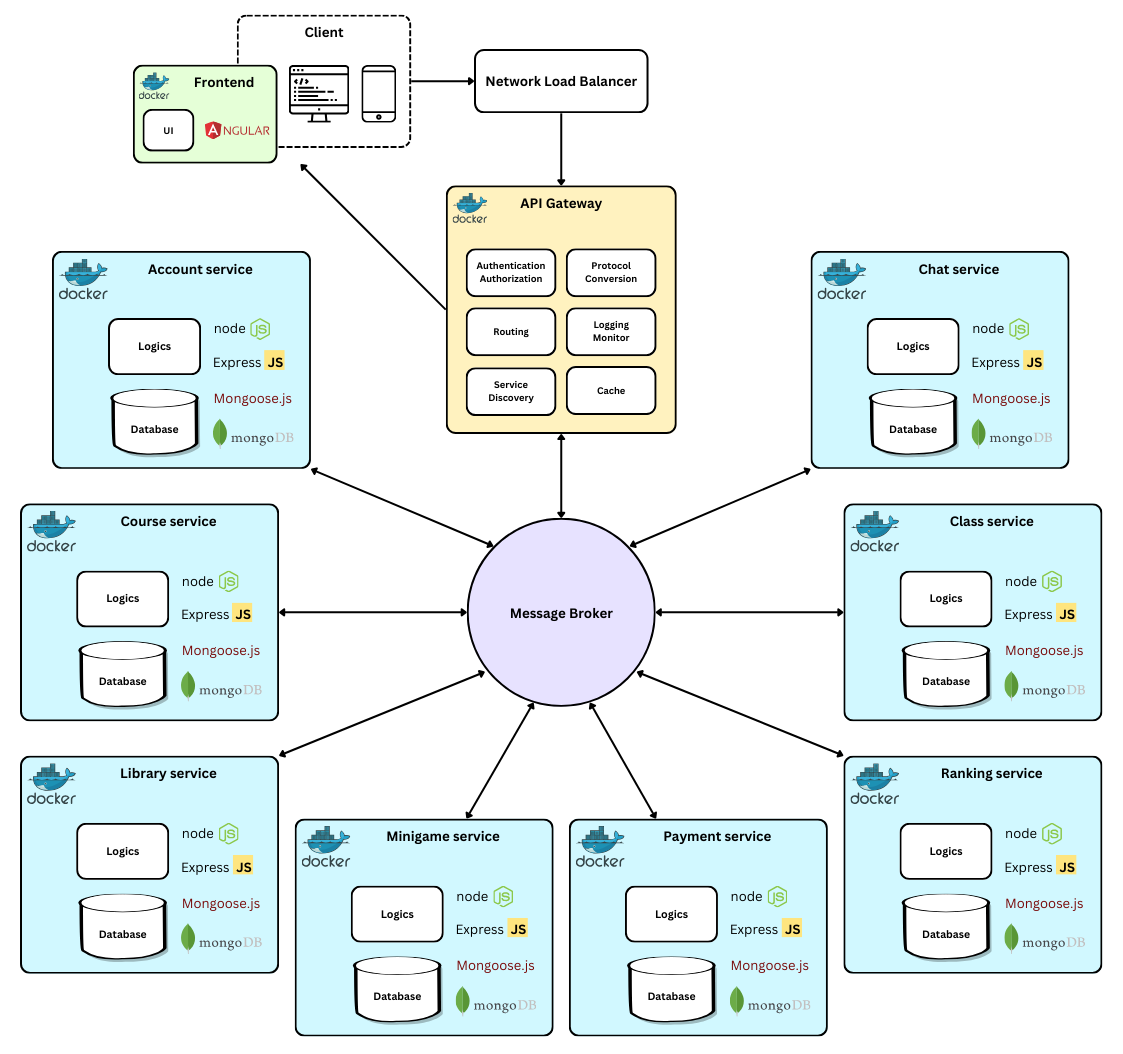
\includegraphics[width=1.0\linewidth]{images/architecture-description.png}
	\caption{RadiantIQ - Architecture description diagram}
	\label{fig:architecture-description}
\end{figure}

\subsection{Architectural Components}

\subsubsection{Frontend}
\begin{itemize}
    \item \textbf{Technology Stack}: Angular, NgBootstrap
    \item \textbf{Description}: The frontend is responsible for delivering a responsive and interactive user interface. It communicates with the backend services through the API Gateway.
\end{itemize}

\subsubsection{API Gateway}
\textbf{Responsibilities}:
\begin{itemize}
    \item \textbf{Authentication and Authorization}: Verifies user credentials and permissions.
    \item \textbf{Routing}: Forwards requests to the appropriate backend services.
    \item \textbf{Service Discovery}: Determines the location of microservices.
    \item \textbf{Protocol Conversion}: Converts protocols (e.g., HTTP to WebSockets).
    \item \textbf{Logging and Monitoring}: Tracks and logs requests for monitoring and debugging.
    \item \textbf{Caching}: Stores frequently accessed data to improve performance.
\end{itemize}

\subsubsection{Microservices}
Each microservice is designed to handle a specific domain within the RadiantIQ platform. They are developed using Node.js and Express, and use MongoDB for data storage. Each service is deployed in a separate container, ensuring isolation and scalability.

\begin{itemize}
    \item \textbf{Account Service}: Manages user accounts, including registration, login, and profile management.
    \item \textbf{Chat Service}: Handles real-time messaging between users.
    \item \textbf{Class Service}: Manages virtual classrooms, including scheduling and attendance.
    \item \textbf{Course Service}: Manages course content, enrollment, and progress tracking.
    \item \textbf{Library Service}: Provides access to educational resources, materials and allows users to create and share collections.
    \item \textbf{Minigame Service}: Create an environments for external developers to create minigames.
    \item \textbf{Payment Service}: Manages payment processing for course enrollments and other transactions.
    \item \textbf{Ranking Service}: Tracks and displays user rankings and achievements.
\end{itemize}

\subsubsection{Message Broker}
\textbf{Description}: Facilitates communication between microservices using a publish-subscribe model. Ensures that messages are reliably delivered to the appropriate services.

\subsection{Communication Flow}

\begin{enumerate}
    \item \textbf{Client Request}:
    \begin{itemize}
        \item The client (frontend) sends a request to the Network Load Balancer.
        \item The Network Load Balancer forwards the request to the API Gateway.
    \end{itemize}

    \item \textbf{API Gateway Processing}:
    \begin{itemize}
        \item The API Gateway authenticates the request and checks user authorization.
        \item It routes the request to the appropriate service based on the endpoint and request data.
    \end{itemize}

    \item \textbf{Service Interaction via Message Broker}:
    \begin{itemize}
        \item The API Gateway forwards the request to the Message Broker.
        \item The Message Broker directs the request to the corresponding microservice (e.g., Course Service for course-related operations).
    \end{itemize}

    \item \textbf{Inter-service Communication}:
    \begin{itemize}
        \item Services communicate with each other through the Message Broker using GraphQL API. This ensures decoupled and asynchronous communication, enhancing scalability and reliability.
    \end{itemize}

    \item \textbf{Response Handling}:
    \begin{itemize}
        \item The target microservice processes the request and sends the response back to the API Gateway through the Message Broker.
        \item The API Gateway returns the response to the client.
    \end{itemize}
\end{enumerate}

\subsection{Deployment and Scalability}

\begin{itemize}
    \item Each microservice is containerized using Docker, ensuring consistent environments across development, testing, and production.
    \item Services can be independently scaled based on load and performance requirements.
    \item Kubernetes (or another orchestration tool) can be used to manage container deployment, scaling, and load balancing.
    \item Finally the services are deployed on a cloud provider Render.com to expose to the internet.
\end{itemize}

\begin{figure}[H]
	\centering
	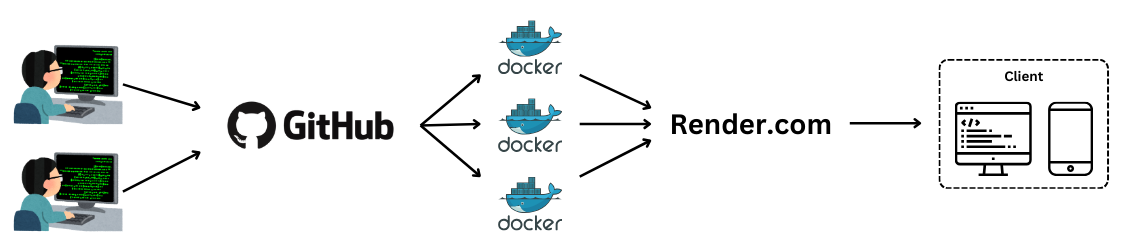
\includegraphics[width=1.0\linewidth]{images/deploy-workflow.png}
	\caption{RadiantIQ - Develop and deploy workflow}
	\label{fig:deploy-workflow}
\end{figure}

\subsection{Monitoring and Maintenance}

\begin{itemize}
    \item \textbf{Logging and Monitoring}: Integrated within the API Gateway and microservices to track performance, errors, and usage patterns.
    \item \textbf{Continuous Integration/Continuous Deployment (CI/CD)}: Using Github and Github Action to automate pipelines for testing and deploying new code changes to ensure rapid and reliable updates.
\end{itemize}
